\begin{figure}[htpb!]
  \begin{center}
  \caption{Mother's Age at First Birth}
  \label{bqFig:NVSSages}
  \includegraphics[scale=0.82]{./../results/nvss/graphs/ageDescriptive.eps} 
  \end{center}
\end{figure}

\vspace{8mm}


\begin{figure}[htpb!]
  \begin{center}
  \caption{Difference in Births: \% Good Season--\% Bad Season (Education)}
  \label{bqFig:diffQ}
  \includegraphics[scale=0.82]{../results/nvss/graphs/birthQdiff.eps}
  \end{center}
  {\footnotesize Note to figure \ref{bqFig:diffQ}: `Young' refers to 25-39 years
  old at first birth.  `Old' refers to 40-45 at first birth.}
\end{figure}


\begin{figure}[htpb!]
  \begin{center}
  \caption{Difference in Births (\% Good Season - \% Bad Season)}
  \label{fig:NVSSbirthsAges}
  \includegraphics[scale=0.8]{./../results/nvss/graphs/birthQdiff_4Ages.eps}
  \end{center}
\end{figure}

\begin{figure}[htpb!]
\begin{center}
\caption{Births per Month (25-39): Northern and Southern Hemisphere Countries}
\label{bqFig:excess}
\includegraphics[scale=1.15]{../results/countries/combinedMonthExcess.eps}
\end{center}
{\footnotesize Note to figure \ref{bqFig:excess}: Each panel is one country.  Bars
represent the difference between expected (evenly spaced) births and actual births.  
Births for USA are 2005-2013, for Chile 2000-2012, for Mexico 2000-2005 and for Spain 
2013.  Earlier births are used for Mexico as reporting can occurr after the date of
the event while for each of the other country data is recorded at the time of birth.  
Average temperatures per month for each country are plotted in appendix figure 
\ref{bqFig:excessTemp}.}
\end{figure}
\vspace{5mm}

\begin{figure}[htpb!]
  \begin{center}
  \centering
  \caption{Proportion of Mothers Reporting any ART}
  \label{bqfig:NVSSART}
  \includegraphics[scale=0.82]{./../results/nvss/graphs/ART.eps}
  \end{center}
  {\footnotesize Note to figure \ref{bqfig:NVSSART}: Questions on ART use are 
  only included in 2012-2013 birth certificate data.}
\end{figure}

\clearpage

\begin{figure}[htpb!]
  \begin{center}
  \centering
  \caption{Proportion of Twins Born by Age}
  \label{fig:NVSSTwins}
  \includegraphics[scale=0.77]{./../results/nvss/graphs/twinPrevalence.eps}
  \end{center}
\end{figure}


\begin{figure}[htpb!]
\caption{Conception and Births: 25-39 Year-olds}
\hspace{8.0cm}\textbf{Realized Season} \vspace{4mm}\\
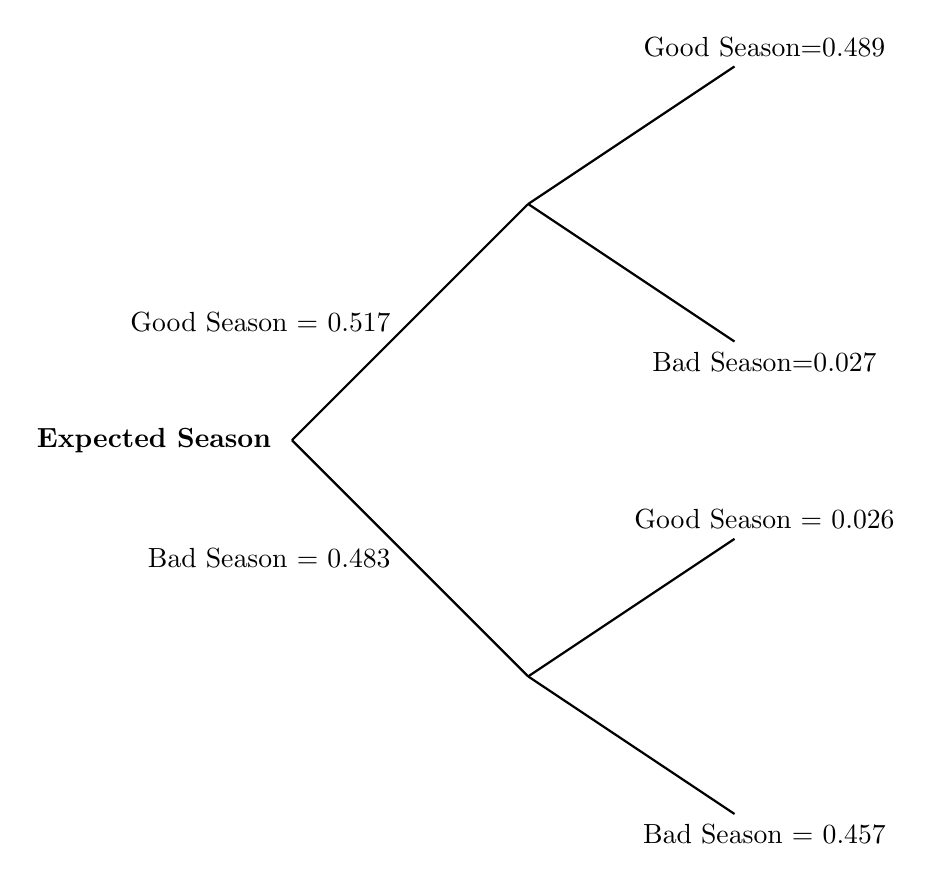
\begin{tikzpicture}[thick,
    level/.style={level distance=3cm},
    level 2/.style={sibling distance=6cm},
    level 3/.style={sibling distance=4cm}
]
\coordinate
child[grow=right, level distance=0pt] {
        child  {
            child {
                node {Bad Season = 0.457}
                edge from parent 
            }
            child {
                node {Good Season = 0.026}
                edge from parent
            }
            edge from parent
            node [left] {Bad Season = 0.483 \ }
        }
        child {
            child {
                node {Bad Season=0.027}
                edge from parent
            }
            child {
                node {Good Season=0.489}
                edge from parent  
            }
            edge from parent 
            node [left] {Good Season = 0.517 \ }
        }
        node [left] {\textbf{Expected Season\ \ }}
    };
\end{tikzpicture}
\end{figure}


\begin{figure}[htpb!]
\caption{Conception and Births: 40-45 Year-olds}
\hspace{8.0cm}\textbf{Realized Season} \vspace{4mm}\\
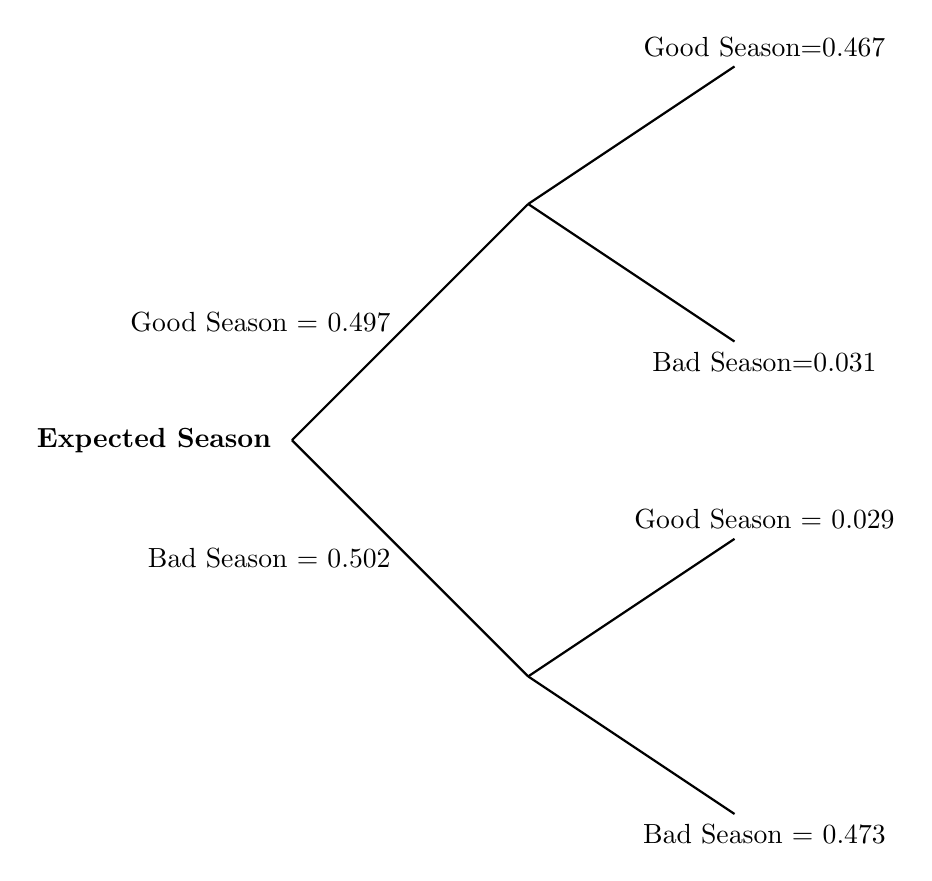
\begin{tikzpicture}[thick,
    level/.style={level distance=3cm},
    level 2/.style={sibling distance=6cm},
    level 3/.style={sibling distance=4cm}
]
\coordinate
child[grow=right, level distance=0pt] {
        child  {
            child {
                node {Bad Season = 0.473}
                edge from parent 
            }
            child {
                node {Good Season = 0.029}
                edge from parent
            }
            edge from parent
            node [left] {Bad Season = 0.502 \ }
        }
        child {
            child {
                node {Bad Season=0.031}
                edge from parent
            }
            child {
                node {Good Season=0.467}
                edge from parent  
            }
            edge from parent 
            node [left] {Good Season = 0.497 \ }
        }
        node [left] {\textbf{Expected Season\ \ }}
    };
\end{tikzpicture}
\end{figure}


\begin{figure}[htpb!]
\begin{center}
  \centering
  \caption{Good Season by State (Young)}
  \includegraphics[scale=0.34]{./../results/nvss/graphs/maps/young.png}
  \label{fig:mapYoung}
\end{center}
\end{figure}

\begin{figure}[htpb!]
\begin{center}
  \centering
  \caption{Good Season by State (Old)}
  \includegraphics[scale=0.34]{./../results/nvss/graphs/maps/old.png}
  \label{fig:mapOld}
\end{center}
\end{figure}

\begin{figure}[htpb!]
\begin{center}
  \centering
  \caption{Temperature and good Quarter: Young (Spain)}
  \includegraphics[scale=0.8]{./../results/spain/graphs/youngTempCold.eps}
  \label{fig:mapYoung}
\end{center}
\end{figure}
\clearpage

\begin{figure}[htpb!]
\begin{center}
  \centering
  \caption{Temperature and good Quarter: Old (Spain)}
  \includegraphics[scale=0.8]{./../results/spain/graphs/oldTempCold.eps}
  \label{fig:mapOld}
\end{center}
\end{figure}

\begin{figure}[htpb!]
\centering
\caption{Child quality: Birthweight (grams)}
\label{QBwt}
\includegraphics[scale=0.8]{../results/nvss/graphs/AllQuality_birthweight_.eps}
\end{figure}
\vspace{1cm}

\begin{figure}[htpb!]
\centering
\caption{Child quality: Birthweight (grams)}
\label{QApgar}
\includegraphics[scale=0.8]{../results/nvss/graphs/Quality_birthweight_.eps}
\end{figure}
\vspace{1cm}



